\begin{surferPage}[Кайлей]{Кубика Кайлея}
Эта кубика (т.е. поверхность третьей степени) обладает одновременно четырьмя сингулярностями в форме двойного конуса. Название происходит от имени ученого Артура Кайлея, занимавшегося исследованием кубических поверхностей. 

    
Но первым таким исследователем был Людвиг Шлефли, именно он в 1863 году начал систематически изучать такие поверхности, поставив вопрос о том, какие типы сингулярностей имеются. Например, в его работах можно прочесть, почему на одной кубической поверхности одновременно не может быть более $4$ особых точек (сингулярностей), т.е. $\mu(3)=4$. 
    
Феликс Христиан Клейн в 1900-х гг. также исследовал кубические поверхности на наличие их возможных форм; его идея состояла в том, чтобы ответить на вопрос, базируясь на кубике Кайлея, путем небольших преобразований: благодаря расширениям, разверткам двойного конуса и их объединению можно, действительно, получить все другие тела, например, 
    \vspace{0.3cm}
     \begin{center}
      \vspace{-0.2cm}
      \begin{tabular}{@{}c@{\ }c@{\ }c@{\ }c@{}}
        \begin{tabular}{@{}c@{}}
          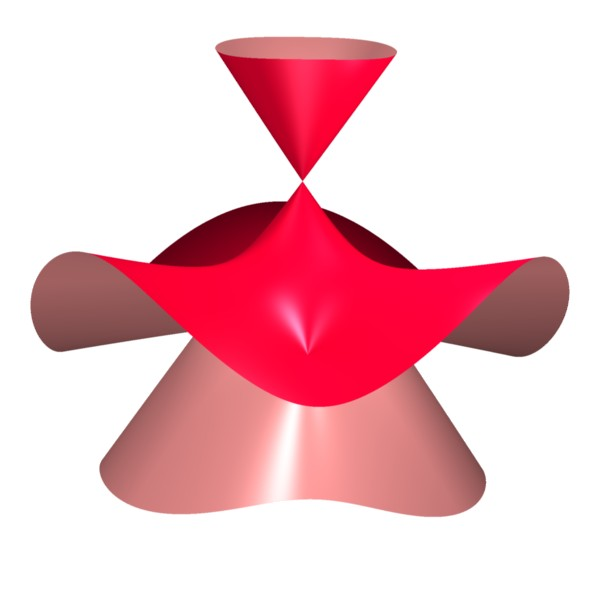
\includegraphics[width=1.35cm]{./../../common/images/cayley_cubic_0}
        \end{tabular}
        &
        \begin{tabular}{@{}c@{}}
          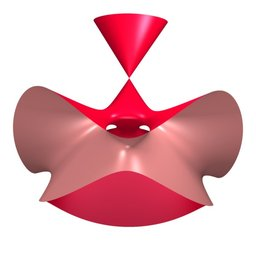
\includegraphics[width=1.35cm]{./../../common/images/cayley_cubic_1}
        \end{tabular}
        &
        \begin{tabular}{@{}c@{}}
          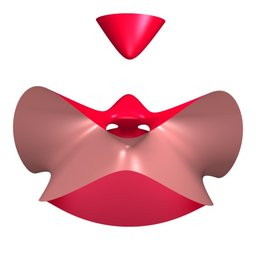
\includegraphics[width=1.35cm]{./../../common/images/cayley_cubic_2}
        \end{tabular}
        &
        \begin{tabular}{@{}c@{}}
          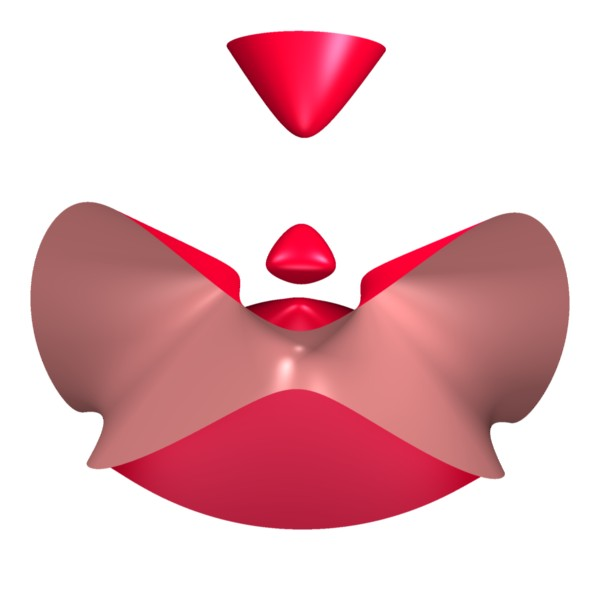
\includegraphics[width=1.35cm]{./../../common/images/cayley_cubic_3}
        \end{tabular}
      \end{tabular}
    \end{center}
\end{surferPage}
